\documentclass[oneside]{report}
\usepackage{geometry}
\usepackage[english]{babel}
\usepackage[final]{graphicx}
\usepackage{amsmath}
\setlength{\parindent}{0pt}
\usepackage{float}
%\counterwithout{section}{chapter}
\usepackage{fullpage}
%\geometry{hmargin=20mm, vmargin=20mm}

\usepackage[backend=bibtex,
    natbib=true,
    style=numeric,
    sorting=none]{biblatex}
\addbibresource{lms464.bib} 

\begin{document}
\section*{Application Description}

Synaptic membranes are unique mammalian membranes \cite{Bozek2015}, composed of lipids that include a high fraction of omega-3 polyunsaturated fatty acids (PUFAs) and cholesterol \cite{Isolated1969,Breckenridge1973,Ingolfsson2017}.  Pathologies that result in altered lipid composition of the neuronal membrane can have devastating effects, including Alzheimer's Disease, Parkinson's Disease, schizophrenia, and epilepsy \cite{MuralikrishnaAdibhatla}. As an example,  %people who suffered from Alzheimer's disease often have much lower levels of cholesterol in the membranes of their hippocampus than people without neurodegenerative disorders, and 
one of the most significant Alzheimer's disease risk factors is the $\epsilon$4 mutation in apolipoprotein E, which mediates cholesterol delivery to neurons.\cite{liu2013}\\

A major obstacle in understanding and treating all lipid-associated neurological disorders is that we do not understand how changing the lipid composition changes the behavior of neuronal membranes.  Molecular simulations are promising but have been limited in size and complexity.  The total synaptic apposition area is about 0.1-4$\mu$m$^{2}$\cite{yeow1991} with hundreds of lipids and proteins, while simulated membranes using coarse-grained models are about $10^{-4}\mu$m$^{2}$, and may contain a handful of lipids and one type of protein (Figure 1). \\

We are requesting an allocation for molecular simulations of neuronal cell membranes that are 100 times larger in area (Figure \ref{fig:Sci}B) and 10 times more complex than previous simulations conducted by any research group. These neuronal membranes will be 0.01 $\mu$m$^{2}$, with 30 species of lipid, 100 proteins, and 8 million particles. \\

\begin{figure}[h]
\begin{center}
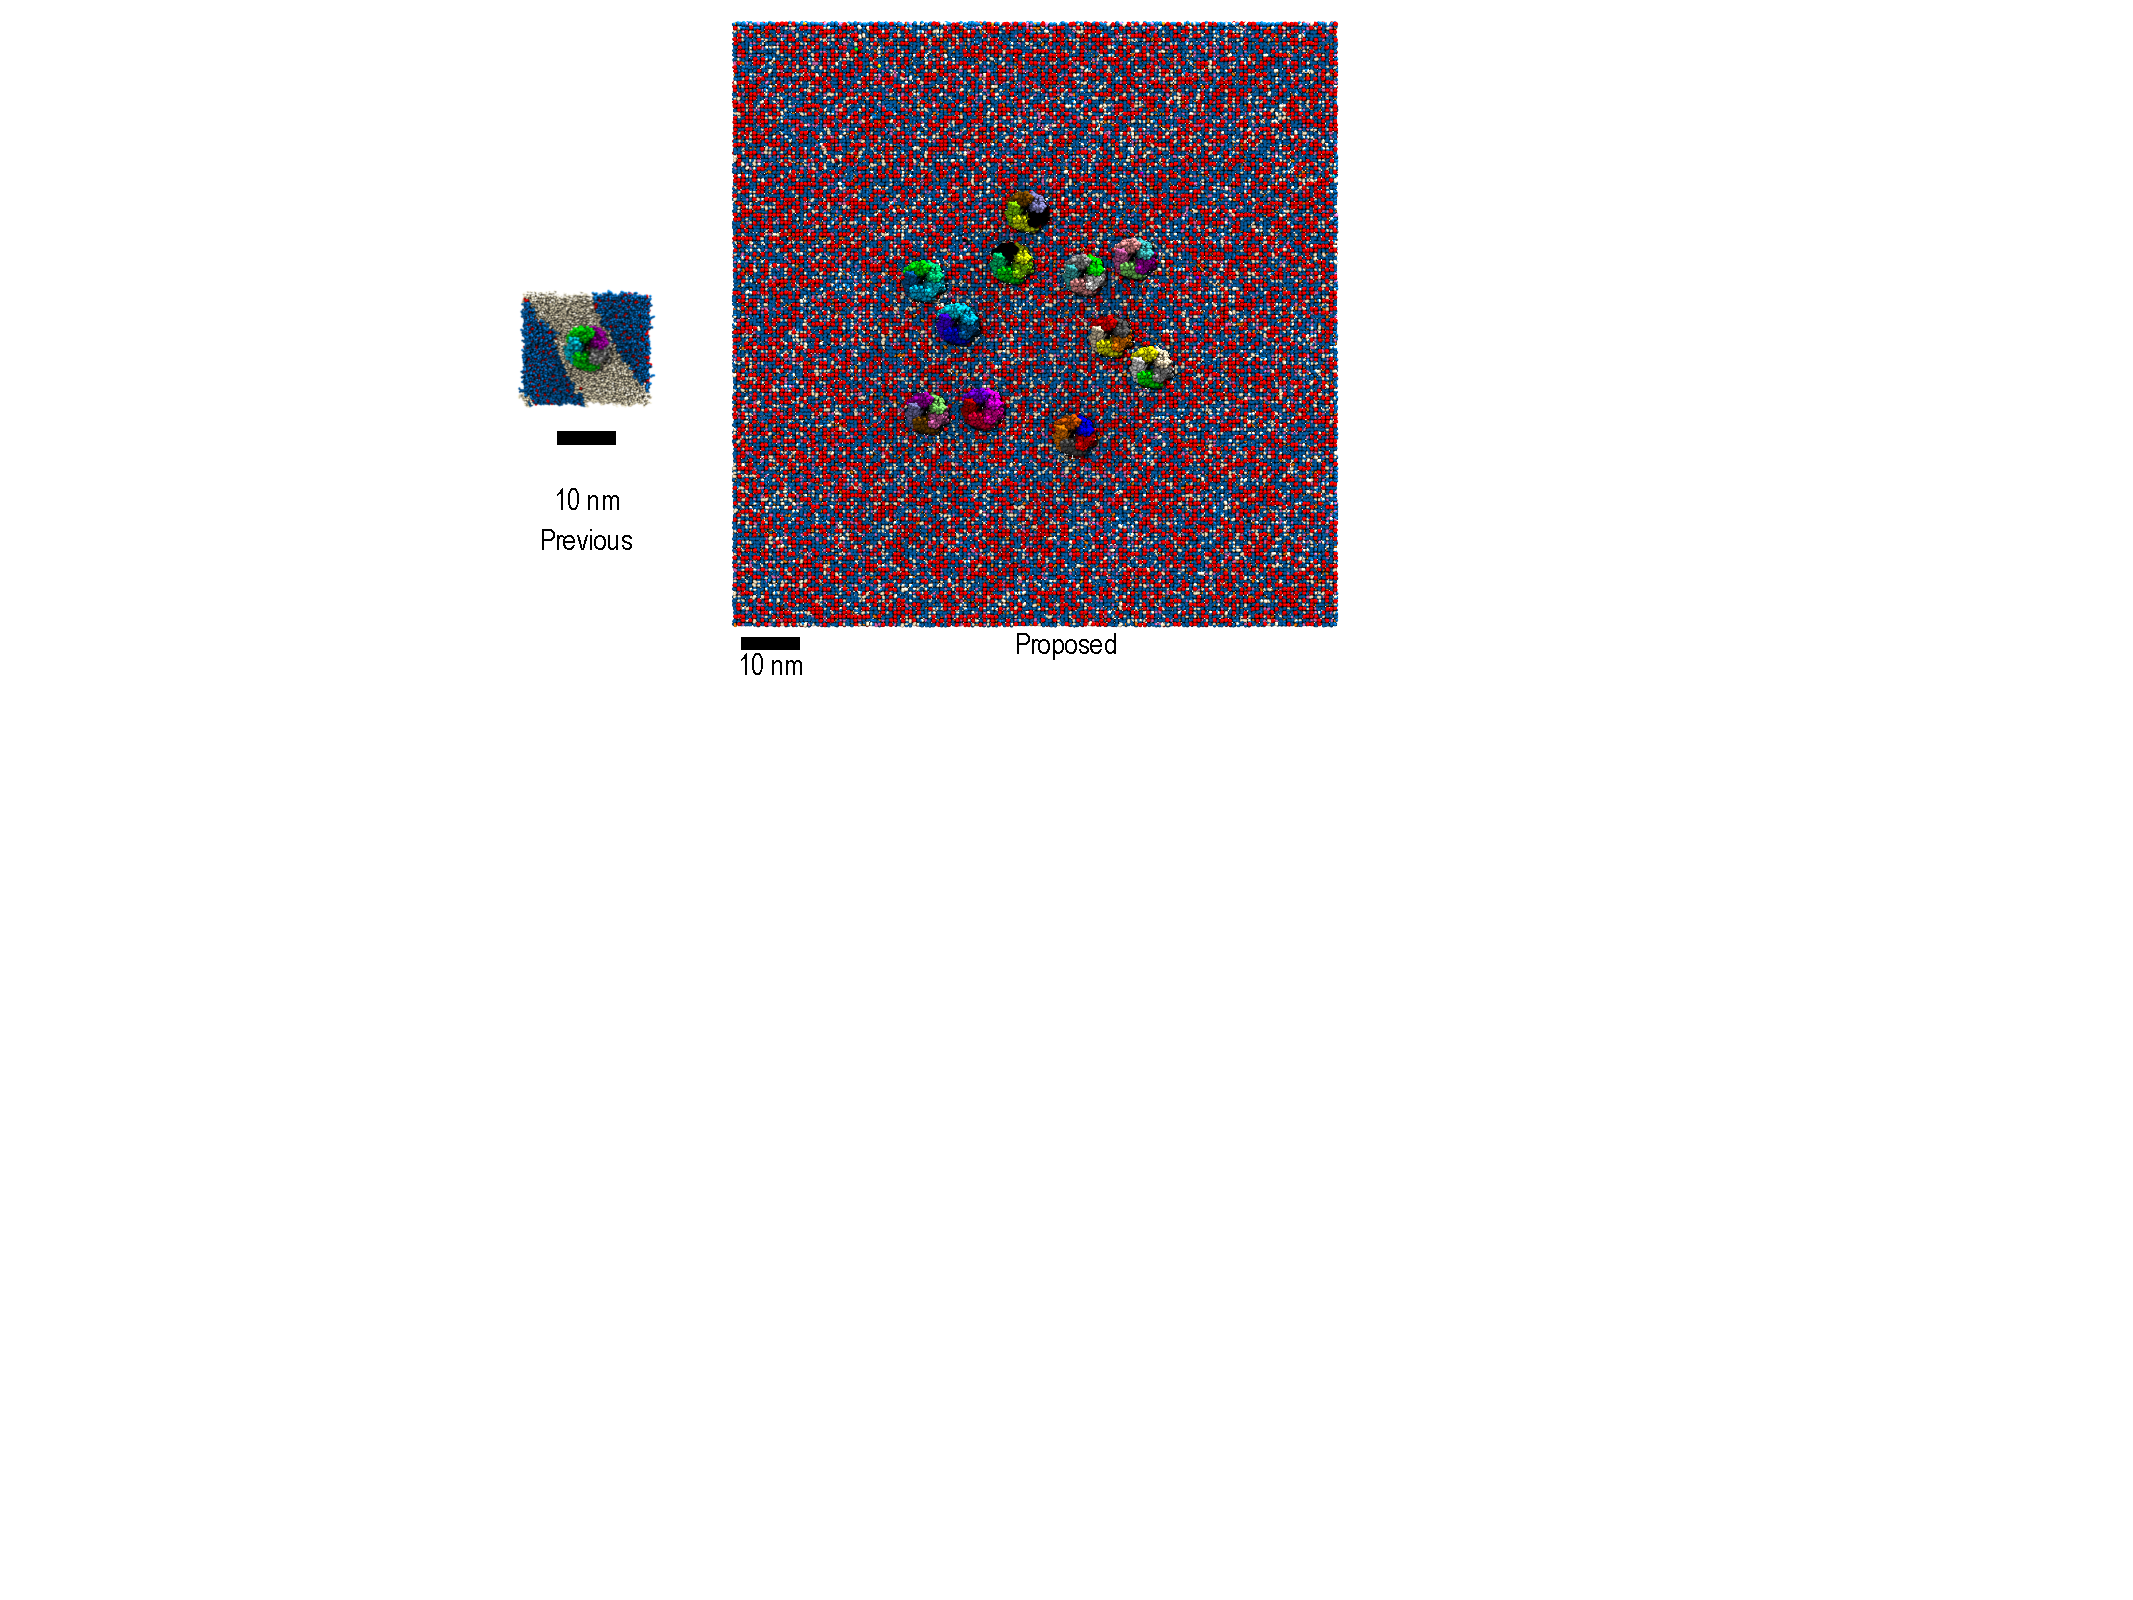
\includegraphics [scale=.4]{Science_Fig2.pdf}
\end{center}
\label{fig:Sci}
\caption{ Left: Previous simulation\cite{Sharp2019} run on Caliburn involving a domain-forming membrane with three different types of lipids and a neuronal ion channel. Right: A membrane of the size planned for simulation, comprising 1-10\% of the area of the post-synaptic membrane, and containing eleven of the same proteins.}
\end{figure}

%This research is motivated by two major questions:
%\begin{itemize}
%    \item Western diets are rich in omega-6 but low in omega-3 PUFAs. Does this lack of omega-3's change the organization of proteins in the post-synaptic membrane?
%    \item Membranes de-mix into two over-arching phases, one rich in cholesterol/saturated fatty acids and the other rich in unsaturated fatty acids. How do these domains change the distribution and density of proteins?
%\end{itemize}

%\subsection*{General Workflow}

{ \bf General Workflow} Our general pipeline is as follows:1) Construct system on local machine. Membranes will contain $\pmb{>30}$ \textbf{lipid species} in a composition similar to rat synapse, and will also contain approximately \textbf{100 proteins} chosen from the most prevalent post-synaptic membrane proteins with available PDB structures. 2) Upload to Caliburn. 3) Run energy minimization and MD simulation using GROMACS 2019.2 \cite{Berendsen1995} for at least 20$\mu$s 4) Analyze using Visual Molecular Dynamics 1.9.3 \cite{HUMP96} and Python3. 
%Initial tests using membranes with $0.01\mu$m$^2$ in area, as in Figure 1B, have shown simulations run well with a time step of $0.02 ps$. The size of these simulations will require approximately  $\pmb{20 \mu s}$ to simulate each, the first $5-10 \mu s$ will be allowing the system to reach equilibrium. 
This research would require running 10 simulations with proteins and multiple lipid compositions, and 4 simulations without proteins , treated as controls. The net simulation time will be $\pmb{\sim 280 \mu s}$. \\

%\subsection*{Software Requirements and Storage.}

{\bf Software Requirements and Storage} The proposed research would utilize \textbf{GROMACS 2019.2 mpi packages } \cite{Berendsen1995} using the MARTINI 2.2\cite{Marrink2007} coarse grained force field.  Initial bench marking projects a single simulation will require 1 TBs of storage. For 14 simulations this would require \textbf{$\sim$ 3.0 TBs} of storage.\\

%\subsection*{Application Readiness}

{\bf Application Readiness} All software required is open-source and available on Caliburn.\\ %Systems lacking proteins can be prepared for simulation before the end of June. Membrane-proteins systems will require  about a month of testing in-order to optimize restraints. Caliburn currently has the software and packages for this research, available.

\section*{Number of requested SUs and storage justification}

{\bf Total number of SUs and storage, job size, scalability}
\begin{figure}[h]
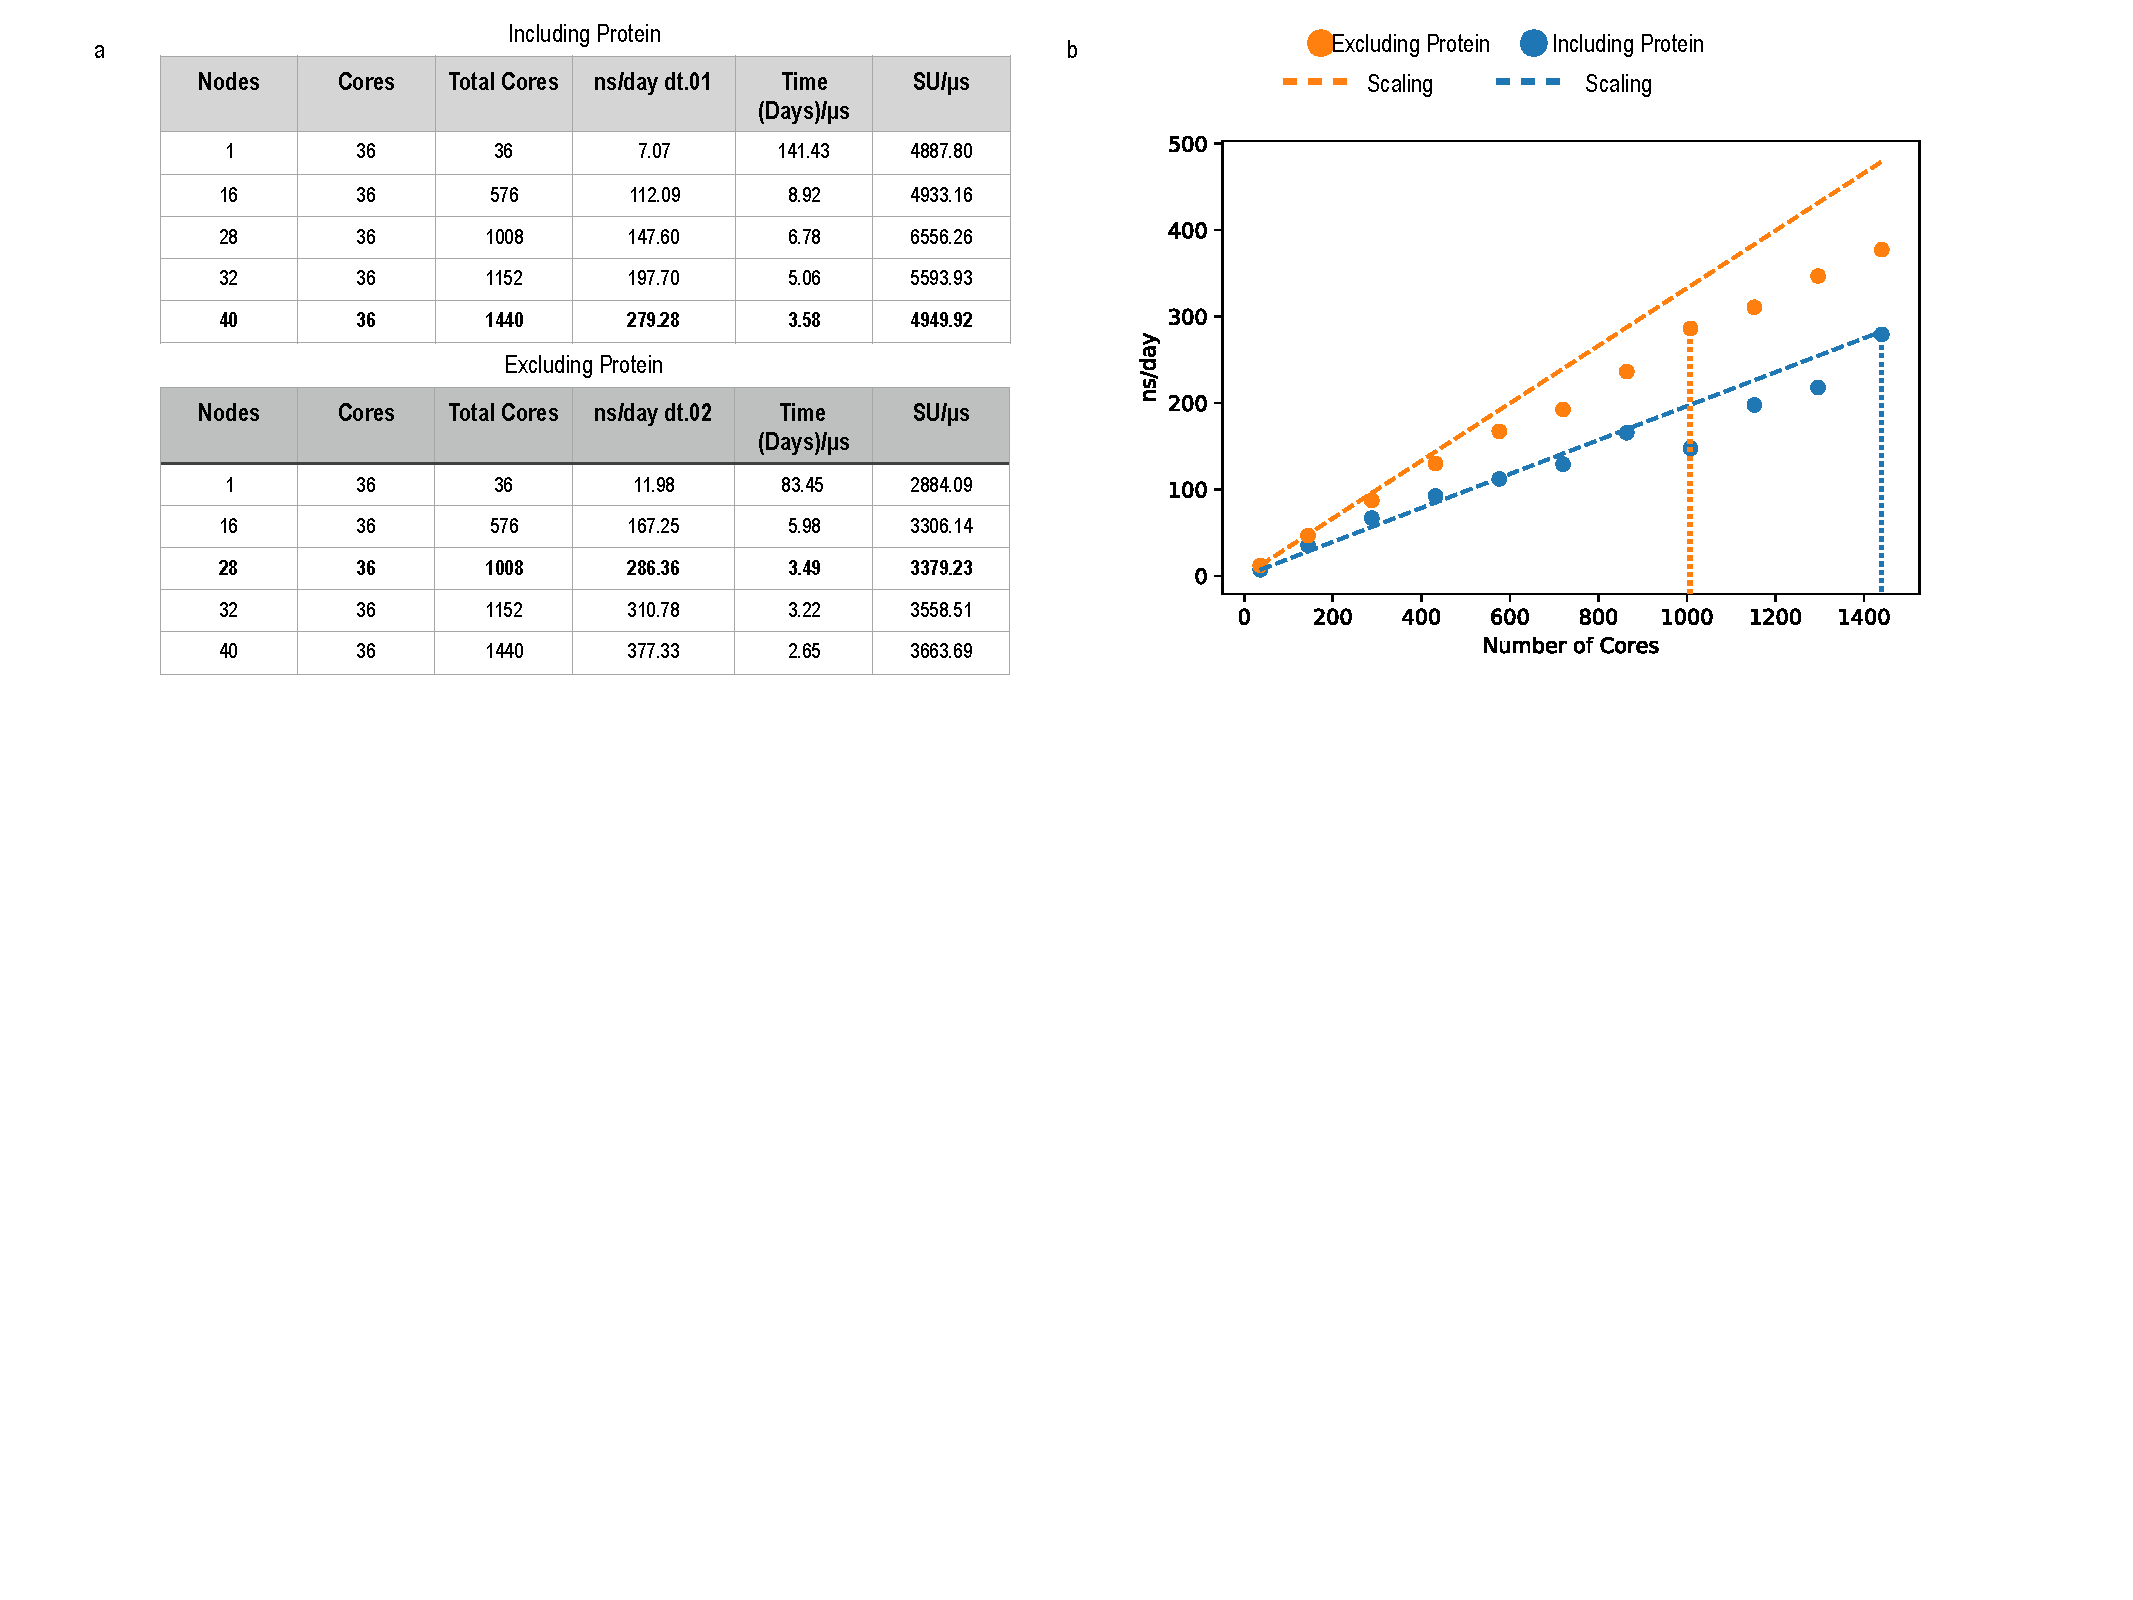
\includegraphics [scale=.5]{SU_Bench.pdf}
\label{fig:SU}
\caption{Projected SU's required for an iteration of membrane simulations with and without proteins. Bench marks are for systems with $\pmb{\> 8,000,000}$ \textbf beads a) Tables show subset of bench marked data. Systems including proteins showed 40 nodes and 36 cores provided the highest efficiency. Systems excluding proteins were tested using 28 cores and 36 nodes. These settings appear optimal to complete simulations within the allotted 6 months allocation. b) Full bench mark set comparing the ns/day to the total number of cores. Lines are associated with optimal node numbers.}
\end{figure}

Using Rutgers Discovery Informatics Institute's Caliburn, \textbf{40 nodes and 36 cores} provided the best scaling for membranes with protein inclusions, and \textbf{28 nodes and 36 cores} for membrane only. We do observe $\sim 17\%$ divergence from expected scaling in membrane only systems, and a divergence for $\sim 1.25\%$ in the membrane-protein systems, while using 40 nodes and 36 cores Figure \ref{fig:SU}. \\

Membranes including proteins SU's:
\[20,000\textrm{ ns x }40\textrm{ nodes x }24\textrm{ hr/day x } 36 \textrm{ cores/node x } 1 \textrm{ SU/hr/node $ \div$ }279.3 \textrm{ ns/day = } \textbf{2,474,960 \textrm{SU}} \]
Membranes excluding proteins SU's:
\[ 20,000\textrm{ ns x }28\textrm{ nodes x }24\textrm{ hr/day x } 36 \textrm{ cores/node x } 1 \textrm{ SU/hr/node $ \div$ }377.3\textrm{ ns/day = } \textbf{2,413,732 \textrm{SU}} \]

For all systems we would need 34,404,528 SU's for this project: 

\[\textrm{Net SU's:  } (10*2,474,960 \textrm{ SU's}) + (4*2,413,732 \textrm{ SU's}) = \textbf{34,404,528 \textrm{ SU's}} \]

Systems are projected to require $\sim$ 4-5 months. to reach 20 $\mu s$. All simulations will produce upwards of $\sim$~1.0 TBs of data. For 14 systems this is a projected {14 TBs of data}, but most will be downloaded to local storage.  We request \textbf{3.0 TB} of working storage on Caliburn for this project.  \\

{\bf Access to Additional Resources}
We have access to Rutgers Office of Advanced Research Computing's Amarel, including maximum priority on 12 nodes. Due to the condominium structure of Amarel, it is not practical to continually run the massively parallel simulations we aim to run here, which requires 28 to 40 nodes. 
\clearpage
\section*{Team Description}
    \begin{itemize}
    	\item PI: Dr. Grace Brannigan
	\begin{itemize}
	\item email address: gracebrannigan@gmail.com
	\item Contact Number: (856)-225-6780
	\item Address: JHSC 213, Rutgers Camden
	\item Campus: Rutgers Camden
	\item School: Rutgers Camden
	\item Department: Physics, CCIB
    \end{itemize}
    \end{itemize}
    Users:
        \begin{itemize}
        		\item Name: Liam Sharp
                \begin{itemize}       
			\item netid: lms464
                    	\item email address: lms464@scarletmail.rutgers.edu
                    	\item Contact Number: (609)-707-0974
                    	\item Address: JHSC 233, Rutgers Camden
                    	\item Campus: Rutgers Camden
                    	\item School: Rutgers Camden
                    	\item Department: CCIB
		\end{itemize}
		\item Name: Jesse Sandberg
	        \begin{itemize}
			\item netid: js2746
                    	\item email address: js2746@scarletmail.rutgers.edu
                    	\item Contact Number: (215)-470-7709
                    	\item Address: JHSC 233, Rutgers Camden
                    	\item Campus: Rutgers Camden
                    	\item School: Rutgers Camden
                    	\item Department: CCIB
	    \end{itemize}
	    \item Name: Tom Joseph
	    \begin{itemize}
	    		\item netid: tj227
                    	\item email address: ttjoseph@gmail.com
                    	\item Contact Number: (856)-571-4266
                    	\item Address: JHSC 233, Rutgers Camden
                    	\item Campus: Rutgers Camden
                    	\item School: Rutgers Camden
                    	\item Department: CCIB
	    \end{itemize}
	    \item Name: Anushriya Subedy
	    \begin{itemize}               
			\item netid: as3190
                    	\item email address: as3190@rutgers.edu
                    	\item Contact Number: (530)-848-2896
                    	\item Address: JHSC 233, Rutgers Camden
                    	\item Campus: Rutgers Camden
                    	\item School: Rutgers Camden
                    	\item Department: CCIB
	    \end{itemize}
	    \item Name: Connor Pitman
	    \begin{itemize}               
			\item netid: csp127
                    	\item email address: csp127@scarletmail.rutgers.edu
                    	\item Contact Number: (302)-893-5914
                    	\item Address: JHSC 233, Rutgers Camden
                    	\item Campus: Rutgers Camden
                    	\item School: Rutgers Camden
                    	\item Department: CCIB
	    \end{itemize}
	    \item Name: Jahmal Ennis
	    \begin{itemize}               
			\item netid: jje63
                    	\item email address: jje63@scarletmail.rutgers.edu
                    	\item Contact Number: (609)-353-7312
                    	\item Address: JHSC 233, Rutgers Camden
                    	\item Campus: Rutgers Camden
                    	\item School: Rutgers Camden
                    	\item Department: CCIB
	    \end{itemize}
	    \item Name: Mark Arcaria
	    \begin{itemize}               
			\item netid: ma1786
                    	\item email address: ma1786@scarletmail.rutgers.edu
                    	\item Contact Number: (215)-778-6251
                    	\item Address: JHSC 233, Rutgers Camden
                    	\item Campus: Rutgers Camden
                    	\item School: Rutgers Camden
                    	\item Department: CCIB
	    \end{itemize}

    \end{itemize}
\printbibliography
\end{document}
